\chapter{Solution}

This chapter describes the complete solution, solving the use cases.
We start with an overview of the solution parts.
Then, we give a detailed description of each part.
\par
The solution consists of four projects, which will form the resulting Blazor website containing PHP scripts.
In Figure \ref{img13:infrastructure}, we can see these projects as green rectangles.
The \textit{Server} project references \textit{Blazor App}, containg a part of the website, and \textit{Peachpie.Blazor}, containing an additional support code.
The server cares about serving the Blazor website and its Static Web Assets.
The next project is our library containing an API for including PHP scripts to the website.
There are \texttt{PhpComponent} and \texttt{PhpScriptProvider}, mentioned earlier, together with additional code support necessary for the correct functionality.
There is the Blazor App project, which becomes the environment for running PHP scripts in a browser.
The project references \textit{PHP scripts} and \textit{Peachpie.Blazor}, which content is used to maintain PHP scripts.
We can see the user's defined scripts as .NET project compiled by Peachpie in \textit{PHP scripts}.
\textit{Blazor App} injects the scripts using the components.
\par
The first section aims at \texttt{PhpComponent}.
It introduces the implementation problems connected to creating render demanding applications and solves them.
The second section talks about \texttt{PhpScriptProvider}.
It suggests a convenient way how to include the scripts into a browser, and it presents the component design.
The last section aims at the server settings.
\par
\begin{figure}[!b]\centering
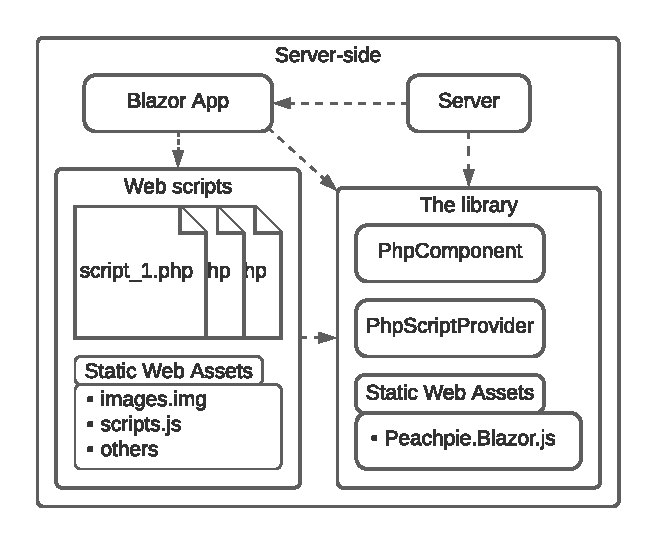
\includegraphics[scale=0.9]{./img/SolutionInfrastructure}
\caption{The solution infrastructure. Green rectangles represent projects. Arrows represent a references.}
\label{img13:infrastructure}
\end{figure} 

\section{PhpComponent}

fasdf
\change[inline]{Problem struct creation in BuildRenderTree}
\change[inline]{PhpComponent structure}
\change[inline]{Additional API for tag, attributes, + rendering + timer}
\change[inline]{Javascript interop}

\section{PhpScriptProvider}

\change[inline]{Division into functionalities (Router, ScriptProvider, Script)}
\change[inline]{Common things(Script finding,rendering, context, Context save, Using forms, files, parsing url)}
\change[inline]{Router navigating}
\change[inline]{ScriptProvider navigating}
\change[inline]{Script navigating}

\section{Server}
\change[inline]{serving web static assets}